\documentclass[11pt, a4paper]{article}

%========================================================================================
% PREAMBLE (Matched to Individual Plan)
%========================================================================================
\usepackage{geometry}
\usepackage{hyperref}
\usepackage{fancyhdr}
\usepackage{amsmath}
\usepackage{enumitem}
\usepackage{tikz}
\usepackage{array}
\usepackage{titlesec}
\usetikzlibrary{positioning, arrows.meta, fit, backgrounds, calc}

\usepackage[utf8]{inputenc}
\usepackage[T1]{fontenc}

\geometry{a4paper, margin=1in}
\setlength{\headheight}{14pt}

\pagestyle{fancy}
\fancyhf{}
\fancyhead[L]{Master's Thesis Pre-Study: Adaptive Hybrid RAG}
\fancyfoot[C]{\thepage}
\renewcommand{\headrulewidth}{0.4pt}
\renewcommand{\footrulewidth}{0.4pt}

\hypersetup{
    colorlinks=true,
    linkcolor=black,
    urlcolor=blue,
}

\begin{document}

%========================================================================================
% TITLE BLOCK
%========================================================================================
\title{
    \textbf{Adaptive Hybrid RAG: Optimizing the Efficiency-Accuracy Trade-off via Learned Query Routing} \\
    \vspace{0.5em}
    \large Pre-Study
}

\author{
    Dante Wesslund \\
    dantew@kth.se
}

\date{March 2026}

\maketitle
\hrule
\vspace{1cm}

%========================================================================================
% CONTENT
%========================================================================================

\section{Introduction}

This pre-study is written as the literature- and method-oriented foundation for the master's thesis on adaptive routing for Hybrid Retrieval-Augmented Generation (RAG). In accordance with the KTH assignment, the document focuses on theoretical background, method choice, and the rationale for the selected thesis direction. The intention is not to claim that the final thesis contribution has already been demonstrated, but to justify why the problem is relevant, why the proposed method is appropriate, and why the work is feasible within the degree-project timeframe.

The core thesis problem is straightforward to state but non-trivial to solve: when should a RAG system use a cheap vector-based retrieval path, and when should it escalate to a more expensive graph-enhanced retrieval path? This is a practical question in industrial RAG systems, but it is also a research question about conditional computation, learned routing, and the interaction between retrieval complexity and query semantics.

The project is motivated by two observations. First, vector retrieval is often sufficient for straightforward factual questions, while graph-enhanced retrieval is more useful for comparison, disambiguation, and multi-hop reasoning. Second, always using the most expensive retrieval strategy is wasteful if a meaningful subset of queries can be answered correctly with cheaper retrieval. The thesis therefore studies whether a learned router can predict the \emph{Minimum Viable Retrieval Mode} for a query before retrieval is executed.

\section{Background and Problem Motivation}

RAG was introduced as a method for combining parametric language-model knowledge with non-parametric memory retrieved from an external corpus \cite{lewis2020rag}. In practice, RAG is now the standard design for grounding large language models in private or frequently changing data. However, basic RAG systems are usually built on vector similarity search over text chunks. This works well for many local factual questions, but it has clear limitations when the answer depends on linking facts across documents, following relationships between entities, or comparing attributes that are distributed across different parts of the corpus.

Hybrid and graph-based retrieval methods try to address these weaknesses by enriching vector retrieval with structured relationships. LightRAG is especially relevant here because it exposes multiple retrieval modes in one framework, including a relatively cheap \emph{Naive} mode and a more expensive \emph{Mix} mode that combines vector retrieval and graph traversal \cite{lightrag2024}. This makes it an attractive experimental substrate for studying routing, because the system already contains the exact cost--accuracy trade-off that the thesis wants to optimize.

The problem is particularly relevant in industrial settings such as Ericsson. Internal technical repositories are large, heterogeneous, and absent from public model pretraining. In such settings, RAG is needed for grounding, but graph-style retrieval and repeated large-model calls can become costly at scale. A static policy that always uses the strongest retrieval mode may improve answer quality, but it also creates systematic overuse of expensive computation. This is the practical inefficiency that motivates the thesis.

\section{Literature Review}

\subsection{RAG, Hybrid Retrieval, and Graph-Based Reasoning}

The original RAG formulation established the broader pattern of retrieving documents and conditioning a generator on retrieved evidence \cite{lewis2020rag}. Since then, the field has moved from simple passage retrieval toward increasingly structured retrieval pipelines. The motivation is consistent across systems: purely local nearest-neighbor retrieval often struggles when reasoning requires composition across multiple pieces of evidence.

This has led to growing interest in graph-augmented and knowledge-structured retrieval. GraphRAG is an especially visible example, showing how graph construction and community-level summarization can improve question answering and corpus-level sensemaking over private document collections \cite{edge2024graphrag}. Related knowledge-graph QA work such as QA-GNN likewise demonstrates that explicitly structured reasoning can help language-model-based QA systems when the answer depends on graph relationships rather than isolated passages \cite{yasunaga2021qagnn}. These lines of work support the thesis motivation: there is a meaningful class of questions for which structured retrieval is not merely an implementation detail, but part of the reasoning mechanism.

LightRAG is especially relevant because it aims to combine simplicity with a richer retrieval mechanism \cite{lightrag2024}. For this thesis, LightRAG is not treated as the theoretical contribution in itself, but as the engineering environment in which the routing problem becomes experimentally tractable. It provides:
\begin{itemize}[label=--]
    \item a vector-only mode suitable as a low-cost baseline,
    \item a graph-enhanced hybrid mode suitable as a higher-cost baseline,
    \item a shared implementation environment where the retrieval mode changes while much of the surrounding system remains fixed.
\end{itemize}

This is important methodologically. If the router is to learn a meaningful decision boundary, the difference between the two actions should be as controlled as possible. LightRAG offers a realistic, but still sufficiently clean, instantiation of that setting.

\subsection{Multi-Hop Benchmarks and Benchmark Choice}

The benchmark landscape also matters for this thesis. HotpotQA established an influential benchmark for explainable multi-hop question answering by providing supporting facts and questions that require reasoning across multiple Wikipedia documents \cite{yang2018hotpotqa}. However, later work has argued that some multihop datasets permit shortcut solutions that do not always require the intended reasoning process. MuSiQue was proposed partly in response to this problem, with a construction procedure intended to require proper multihop reasoning more reliably \cite{trivedi2022musique}. 2WikiMultihopQA is part of the same broader benchmark family and remains attractive for this thesis because it combines gold answers, supporting evidence, and public reproducibility with a manageable and explicit multihop structure \cite{ho2020twowiki}.

This comparison is important because the thesis is not merely using 2Wiki out of convenience. The benchmark choice is part of the methodological argument. 2Wiki offers enough structure to expose non-trivial retrieval demands, while avoiding the need to construct an entirely new gold QA dataset from raw enterprise documents.

\subsection{Adaptive Retrieval, Routing, and Conditional Computation}

The thesis belongs to a broader family of problems concerned with routing, selective computation, and cost-aware decision making. RouterBench is relevant here because it frames routing as a prediction problem where inputs should be sent to different computational paths depending on expected benefit and cost \cite{hu2024routerbench}. Although RouterBench is not about Hybrid RAG specifically, its conceptual contribution is highly aligned with this thesis: routing is useful when different execution paths have different performance--cost profiles, and when the input contains enough signal to predict which path is appropriate.

There is also directly related work on adaptive retrieval-augmented generation. Adaptive-RAG selects among strategies of different complexity based on question complexity, using a smaller classifier to predict which type of processing is needed \cite{jeong2024adaptiverag}. This work is important for the present thesis because it shows that adaptive retrieval is already recognized as a valid research direction. At the same time, it leaves room for a more specific contribution: the present thesis is not primarily about selecting among no-retrieval, single-step retrieval, and iterative retrieval. Instead, it studies the narrower and practically relevant decision between cheap vector retrieval and more expensive graph-enhanced retrieval inside a controlled Hybrid RAG framework.

The present thesis adapts this logic from \emph{model routing} to \emph{retrieval routing}. Instead of deciding which language model to call, the system decides whether graph-enhanced retrieval is required. This shift matters because it positions the work at a more modular layer of the stack. In principle, the router's output is not ``use LightRAG Mix'' as such, but rather ``this query requires expensive structured retrieval rather than cheap vector retrieval.'' LightRAG is simply the first concrete experimental realization of that decision.

\subsection{Confidence Calibration and Threshold-Based Decisions}

The thesis does not end with a binary classifier. The router is intended to operate with a confidence threshold that can be adjusted to trade efficiency against answer quality. This makes calibration relevant, not just raw classification accuracy. Guo et al. show that modern neural networks can be poorly calibrated even when their predictive accuracy is strong, which is important when model probabilities are used as operational decision signals rather than mere scores \cite{guo2017calibration}. Related work on selective classification formalizes the idea that a model can abstain, defer, or change behavior based on confidence, explicitly trading coverage against risk \cite{geifman2017selective}. This literature motivates the planned threshold sweep in the thesis: the router should be evaluated as a decision policy, not only as a classifier.

\subsection{LLM-as-a-Judge as a Labeling Mechanism}

The thesis uses LLM-as-a-Judge not for open-ended benchmarking, but for assigning the supervision target needed for router training. This still requires methodological care. Zheng et al. show that strong LLM judges can correlate well with human preferences, but they also identify several failure modes including position bias, verbosity bias, and limited reasoning reliability in difficult cases \cite{zheng2023llmjudge}. This literature does not rule out judge-based supervision; rather, it shows that LLM judges should be treated as fallible evaluation instruments whose outputs must be grounded carefully. For this thesis, that means the Judge is anchored in benchmark answer and evidence rather than asked to invent truth from scratch.

\subsection{Why an Encoder-Only Router is a Plausible Choice}

The router itself should be substantially cheaper than the computation it is trying to save; otherwise, the routing layer undermines its own purpose. For that reason, a lightweight encoder-only classifier is a more reasonable first choice than a decoder-only LLM router. BERT-style models are designed for bidirectional text understanding and remain strong baselines for classification tasks \cite{devlin2019bert}. More recent comparisons between encoder-only and decoder-only models further support the idea that encoder-only architectures remain attractive when the task is classification rather than free-form generation, especially when efficiency is important \cite{benayas2024encoder}. ModernBERT is particularly relevant because it is explicitly positioned as a modern, fast, memory-efficient bidirectional encoder with strong downstream classification performance and long-context support \cite{warner2024modernbert}.

This makes an encoder-only router methodologically appropriate for three reasons:
\begin{itemize}[label=--]
    \item \emph{Inference cost:} Encoder-only models are much cheaper to run than decoder LLMs at routing time.
    \item \emph{Task fit:} The router's task is to classify whether graph retrieval is required from the query text alone.
    \item \emph{Transfer from pretraining:} Bidirectional pretraining provides a strong starting point for recognizing semantic cues such as comparison structure, entity interaction, and compositional phrasing.
\end{itemize}

The thesis therefore treats a model such as ModernBERT-base as a practical and theoretically justified candidate. The argument is not that encoder-only models are universally best, but that they are the right first method for a speed-sensitive routing layer.

\section{Method Choice and Thesis Positioning}

\subsection{The Research Claim That Needs to Be Tested}

The central thesis claim is not that LightRAG is good, nor that graph retrieval is always better than vector retrieval. Instead, the claim is that \emph{retrieval complexity is predictable enough from the query text that a lightweight router can improve the efficiency--accuracy trade-off relative to static retrieval policies}.

This claim decomposes into three subclaims:
\begin{enumerate}[leftmargin=*, label=\arabic*.]
    \item Some queries require more expensive structured retrieval than others.
    \item This requirement is reflected, at least partially, in the linguistic or semantic properties of the query itself.
    \item A cheap classifier can exploit that signal well enough to save cost without losing too much answer quality.
\end{enumerate}

The pre-study should therefore justify these subclaims at the level of theory and method choice. The full thesis will then test them empirically.

\subsection{Why 2WikiMultihopQA is the Right Main Benchmark}

The selected main benchmark is 2WikiMultihopQA \cite{ho2020twowiki}. This choice is important because benchmark selection determines whether the routing problem is observable in a clean way.

2Wiki is a strong fit for the thesis because it provides:
\begin{itemize}[label=--]
    \item gold questions,
    \item gold short answers,
    \item supporting evidence,
    \item a clearly multi-hop flavor,
    \item a public benchmark that is reproducible and easy to discuss academically.
\end{itemize}

This is a major methodological advantage. The benchmark removes the need to create the QA ground truth from scratch, which would otherwise risk turning the project into a dataset-engineering thesis rather than a routing thesis. The work that remains is the work the thesis \emph{should} focus on: indexing, dual-mode retrieval, LLM-as-a-judge routing labels, supervised training, and offline evaluation.

Another practical advantage is that the dataset can be processed in original sample order. This makes it possible to incrementally index source documents, track exactly which questions are queryable, and grow the experiment in a controlled way. That is valuable both engineering-wise and methodologically.

\subsection{Why Ericsson Data Should Remain an Extension}

Ericsson data is highly relevant to the industrial motivation, but it should not be the main dependency of the thesis. The reason is not lack of importance, but risk management. Internal corpora may require substantial preprocessing, confidentiality handling, and label construction effort. If the thesis depends entirely on such data, the main scientific contribution risks being delayed or diluted by engineering work.

Therefore, the pre-study supports the following priority:
\begin{itemize}[label=--]
    \item use 2WikiMultihopQA as the primary benchmark for the thesis contribution,
    \item use Ericsson data as a potential extension or external validity check if time and access permit.
\end{itemize}

This preserves both academic rigor and industrial relevance. It also aligns with the KTH requirement that the method choice be well motivated and feasible.

\subsection{Why LightRAG is a Good Experimental Testbed}

The router should ideally represent a framework-agnostic decision: \emph{is graph-enhanced retrieval required or not?} However, the thesis still needs a concrete system in which this abstract decision can be measured. LightRAG is a good testbed because it exposes two retrieval modes with a meaningful cost difference while keeping the broader framework stable.

This supports a defensible interpretation:
\begin{itemize}[label=--]
    \item the thesis studies a decision problem that is conceptually broader than one framework,
    \item but evaluates that decision in a concrete implementation where the trade-off is experimentally observable.
\end{itemize}

The pre-study should be honest about this. The thesis cannot claim universal framework generalization from one implementation alone. What it \emph{can} claim is that LightRAG provides a realistic and controlled substrate for studying the retrieval-complexity routing problem.

\subsection{Why LLM-as-a-Judge is the Correct Labeling Strategy}

The final router label needed for training is binary:
\begin{itemize}[label=--]
    \item \texttt{0}: the \emph{Naive} mode was sufficient,
    \item \texttt{1}: the \emph{Mix} mode was required.
\end{itemize}

The crucial point is that these are not labels provided by 2Wiki itself. The benchmark gives QA truth, not routing truth. Therefore, the routing labels must be synthesized after executing both retrieval modes. At the conceptual level, the supervision target is whether low-cost vector retrieval was sufficient or whether more expensive graph-enhanced retrieval was required. In this thesis, that abstract distinction is operationalized concretely through LightRAG's \emph{Naive} and \emph{Mix} modes.

The chosen strategy is to use \emph{strictly} LLM-as-a-Judge for this labeling step. The Judge is given:
\begin{itemize}[label=--]
    \item the query,
    \item the benchmark answer,
    \item the benchmark supporting evidence,
    \item the \emph{Naive} output,
    \item the \emph{Mix} output.
\end{itemize}

The Judge then decides whether the vector-only answer was already sufficient, or whether the graph-enhanced path was required. This is methodologically preferable to heuristic rules, because the routing target is not a simple symbolic function of the benchmark metadata. A question with multiple supporting documents is not automatically a \emph{Mix} case, and a question with apparently simple phrasing is not automatically a \emph{Naive} case. The labeling must therefore depend on the actual retrieval outcomes, not just on dataset structure.

This also preserves the central scientific meaning of the target: the router learns to predict the \emph{minimum viable retrieval mode}, not a proxy defined by hand-crafted rules.

\section{Proposed Thesis Method}

The intended thesis method follows directly from the literature review and method discussion above.

\begin{enumerate}[leftmargin=*, label=\textbf{\arabic*.}]
    \item \textbf{Prepare and index the benchmark corpus.} \\
    Process 2WikiMultihopQA into sample-preserving JSONL, index the source documents into LightRAG, and track which samples are queryable.

    \item \textbf{Execute dual retrieval modes.} \\
    For each queryable sample, run both \emph{Naive} and \emph{Mix}, and log answer text, latency, and other execution metadata.

    \item \textbf{Generate router labels via LLM-as-a-Judge.} \\
    Compare both outputs against the benchmark answer and supporting evidence. The Judge assigns the routing label \texttt{0} or \texttt{1} according to whether \emph{Naive} was sufficient or \emph{Mix} was required.

    \item \textbf{Train a lightweight encoder-only router.} \\
    Fine-tune an encoder-only classifier on the query text to predict whether graph retrieval is needed.

    \item \textbf{Evaluate with offline simulation.} \\
    Apply the router to a held-out split, sweep the decision threshold, and compare the resulting cost--accuracy frontier against static baselines.
\end{enumerate}

\begin{figure}[ht]
\centering
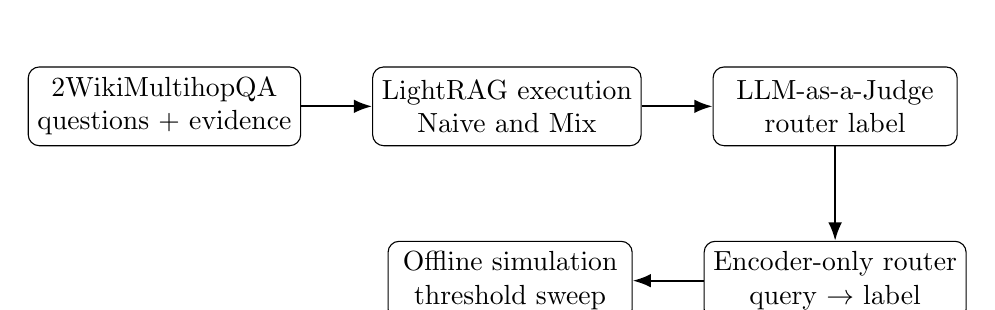
\begin{tikzpicture}[
    node distance=1.2cm and 0.9cm,
    box/.style={draw, rounded corners, align=center, minimum width=3.1cm, minimum height=1cm},
    line/.style={-Latex, thick}
]
    \node[box] (dataset) {2WikiMultihopQA\\questions + evidence};
    \node[box, right=of dataset] (retrieval) {LightRAG execution\\Naive and Mix};
    \node[box, right=of retrieval] (judge) {LLM-as-a-Judge\\router label};
    \node[box, below=of judge] (router) {Encoder-only router\\query $\rightarrow$ label};
    \node[box, left=of router] (eval) {Offline simulation\\threshold sweep};

    \draw[line] (dataset) -- (retrieval);
    \draw[line] (retrieval) -- (judge);
    \draw[line] (judge) -- (router);
    \draw[line] (router) -- (eval);
\end{tikzpicture}
\caption{Planned thesis pipeline. The benchmark provides QA truth, while the routing target is created after dual-mode retrieval and judged sufficiency.}
\end{figure}

\section{Exploratory Feasibility Observations}

Although the final thesis evaluation has not yet been performed, preliminary engineering work already provides a useful feasibility signal. A sample-first 2Wiki processing and indexing pipeline has been implemented in the repository, and LightRAG has been run incrementally on indexed 2Wiki samples.

An exploratory pilot on 30 queryable 2Wiki samples provides an initial motivation for the router problem. Using a rough short-answer containment check over the generated responses, the current implementation produced:
\begin{itemize}[label=--]
    \item 22/30 cases where the \emph{Naive} response contained the gold short answer,
    \item 28/30 cases where the \emph{Mix} response contained the gold short answer,
    \item 6 cases where \emph{Mix} appeared to succeed while \emph{Naive} did not,
    \item 0 cases where \emph{Naive} clearly outperformed \emph{Mix}.
\end{itemize}

At the same time, \emph{Mix} was substantially slower in this exploratory run. Average observed latency was approximately 10.27 seconds for \emph{Naive} and 26.14 seconds for \emph{Mix}. This is not the final evaluation protocol and should not be treated as a formal result. In particular, a containment-style heuristic can partially favor longer answers, which means these pilot numbers should not be interpreted as strong evidence that \emph{Mix} is uniformly superior. The more defensible interpretation is narrower: the two modes are behaviorally different, the cost difference is real, and there are already visible cases where \emph{Mix} appears necessary.

This preliminary observation strengthens the methodological choice made in the pre-study. If the two modes had behaved almost identically, the routing problem would have been much weaker. Instead, the early signal is consistent with the thesis hypothesis that a selective policy could matter.

\section{Risks, Limitations, and Mitigations}

\textbf{Label noise.} The strict LLM-as-a-Judge setup is principled, but judge-based supervision may still introduce noise. This risk is mitigated by grounding the judge in benchmark answers and supporting evidence rather than free-form intuition.

\textbf{Framework dependence.} The thesis is evaluated in LightRAG, which limits direct claims about full framework generality. This is mitigated by framing the contribution at the level of retrieval-complexity routing, while explicitly presenting LightRAG as the experimental instantiation.

\textbf{Benchmark mismatch to industrial data.} Public benchmarks are not the same as Ericsson documentation. This is mitigated by retaining Ericsson as a possible extension and external validity check, without making the thesis scientifically dependent on internal data engineering.

\textbf{Compute and API cost.} Both LightRAG indexing and LLM judging are expensive. This is mitigated by incremental processing, offline simulation after label generation, and a lightweight encoder router rather than a costly LLM router.

\section{Conclusion}

The literature and the current exploratory engineering results both support the thesis direction. The problem is relevant because expensive graph-enhanced retrieval is not always necessary, yet sometimes clearly beneficial. A learned router is therefore a natural research object. An encoder-only classifier is methodologically appropriate because routing is a speed-sensitive classification task. LightRAG is a suitable experimental testbed because it exposes a concrete and controlled cost--accuracy trade-off between \emph{Naive} and \emph{Mix}. 2WikiMultihopQA is a strong primary benchmark because it provides gold QA supervision without forcing the thesis to become a dataset-construction project. Ericsson data remains a valuable extension, but not a prerequisite for a successful and defensible thesis.

In summary, this pre-study concludes that the thesis is methodologically well grounded, feasible within scope, and aligned with both the academic expectations of the KTH course and the practical industrial motivation that initially inspired the work.

\newpage

\begin{thebibliography}{99}

\bibitem{lewis2020rag}
Lewis, P., Perez, E., Piktus, A., Petroni, F., Karpukhin, V., Goyal, N., Kuttler, H., Lewis, M., Yih, W.-t., Rockt\"aschel, T., Riedel, S., \& Kiela, D. (2020).
``Retrieval-Augmented Generation for Knowledge-Intensive NLP Tasks.''
\textit{Advances in Neural Information Processing Systems 33}. \\
\url{https://arxiv.org/abs/2005.11401}

\bibitem{devlin2019bert}
Devlin, J., Chang, M.-W., Lee, K., \& Toutanova, K. (2019).
``BERT: Pre-training of Deep Bidirectional Transformers for Language Understanding.''
\textit{Proceedings of NAACL-HLT 2019}. \\
\url{https://aclanthology.org/N19-1423/}

\bibitem{yang2018hotpotqa}
Yang, Z., Qi, P., Zhang, S., Bengio, Y., Cohen, W. W., Salakhutdinov, R., \& Manning, C. D. (2018).
``HotpotQA: A Dataset for Diverse, Explainable Multi-hop Question Answering.''
\textit{Proceedings of EMNLP 2018}. \\
\url{https://arxiv.org/abs/1809.09600}

\bibitem{trivedi2022musique}
Trivedi, H., Balasubramanian, N., Khot, T., \& Sabharwal, A. (2022).
``MuSiQue: Multihop Questions via Single-hop Question Composition.''
\textit{Transactions of the Association for Computational Linguistics 10}. \\
\url{https://aclanthology.org/2022.tacl-1.31/}

\bibitem{hu2024routerbench}
Hu, Q., et al. (2024).
``RouterBench: A Benchmark for Multi-LLM Routing System.''
\textit{arXiv preprint arXiv:2403.12031}. \\
\url{https://arxiv.org/abs/2403.12031}

\bibitem{jeong2024adaptiverag}
Jeong, S., Baek, J., Cho, S., Hwang, S. J., \& Park, J. C. (2024).
``Adaptive-RAG: Learning to Adapt Retrieval-Augmented Large Language Models through Question Complexity.''
\textit{Proceedings of NAACL 2024}. \\
\url{https://arxiv.org/abs/2403.14403}

\bibitem{benayas2024encoder}
Benayas, A., et al. (2025).
``A comparative analysis of encoder only and decoder only models in intent classification and sentiment analysis: navigating the trade-offs in model size and performance.''
\textit{Language Resources \& Evaluation 59, 2007--2030 (2025)}. \\
\url{https://doi.org/10.1007/s10579-024-09796-y}

\bibitem{warner2024modernbert}
Warner, B., Chaffin, A., Clavi\'e, B., Weller, O., Hallstr\"om, O., Taghadouini, S., Gallagher, A., Biswas, R., Ladhak, F., Aarsen, T., Cooper, N., Adams, G., Howard, J., \& Poli, I. (2024).
``Smarter, Better, Faster, Longer: A Modern Bidirectional Encoder for Fast, Memory Efficient, and Long Context Finetuning and Inference.''
\textit{arXiv preprint arXiv:2412.13663}. \\
\url{https://arxiv.org/abs/2412.13663}

\bibitem{lightrag2024}
Guo, Z., et al. (2024).
``LightRAG: Simple and Fast Retrieval-Augmented Generation.''
\textit{arXiv preprint arXiv:2410.05779}. \\
\url{https://arxiv.org/abs/2410.05779}

\bibitem{edge2024graphrag}
Edge, D., Trinh, H., Cheng, N., Bradley, J., Chao, A., Mody, A., Truitt, S., Metropolitansky, D., Ness, R. O., \& Larson, J. (2024).
``From Local to Global: A Graph RAG Approach to Query-Focused Summarization.''
\textit{Microsoft Research preprint}. \\
\url{https://arxiv.org/abs/2404.16130}

\bibitem{yasunaga2021qagnn}
Yasunaga, M., Ren, H., Bosselut, A., Liang, P., \& Leskovec, J. (2021).
``QA-GNN: Reasoning with Language Models and Knowledge Graphs for Question Answering.''
\textit{Proceedings of NAACL-HLT 2021}. \\
\url{https://aclanthology.org/2021.naacl-main.45/}

\bibitem{ho2020twowiki}
Ho, X., et al. (2020).
``Constructing A Multi-hop QA Dataset for Comprehensive Evaluation of Reasoning Steps.''
\textit{Proceedings of COLING 2020}. \\
\url{https://aclanthology.org/2020.coling-main.580/}

\bibitem{guo2017calibration}
Guo, C., Pleiss, G., Sun, Y., \& Weinberger, K. Q. (2017).
``On Calibration of Modern Neural Networks.''
\textit{Proceedings of ICML 2017}. \\
\url{https://proceedings.mlr.press/v70/guo17a.html}

\bibitem{geifman2017selective}
Geifman, Y., \& El-Yaniv, R. (2017).
``Selective Classification for Deep Neural Networks.''
\textit{arXiv preprint arXiv:1705.08500}. \\
\url{https://arxiv.org/abs/1705.08500}

\bibitem{zheng2023llmjudge}
Zheng, L., Chiang, W.-L., Sheng, Y., Zhuang, S., Wu, Z., Zhuang, Y., Lin, Z., Li, Z., Li, D., Xing, E. P., Zhang, H., Gonzalez, J. E., \& Stoica, I. (2023).
``Judging LLM-as-a-Judge with MT-Bench and Chatbot Arena.''
\textit{NeurIPS 2023 Datasets and Benchmarks Track}. \\
\url{https://arxiv.org/abs/2306.05685}

\end{thebibliography}

\end{document}
